\documentclass[../../main.tex]{subfiles}

\graphicspath{{images/WebApp/}{../../images/WebApp/}}
\begin{document}
\subsection{Webapplikation}
In diesem Kapitel wird auf die Implementierung der technischen Komponente 'Web Applikation' eingegangen. Die Webapplikation wurde am Anfang des Entwicklungsprozess eingeführt und ist somit nicht in Pren1 dokumentiert. 
\subsubsection{Anforderung}

Ziel und Zweck der Applikation ist es eine zentrale Übersicht der einzelnen Module / Komponente zu erhalten und diese zu testen. Somit fungiert die WebApp als Testing/Monitoring Komponente und ist für den Ablauf des Controlflows irrelevant. Der Zug kann mittels Startknopf über das Webinterface gestartet werden.

\paragraph{Anforderungen}
\begin{itemize}
    \item Übersicht
      \subitem Heartbeat
      \subitem Informationen zu Zug \& Fahrt
    \item Module testen
    \item Fahrt starten
\end{itemize}

\subsubsection{Lösung}
Der Client ist eine klassische Kombination aus html \& javascript. Dieser spricht über eine Rest API mit unserem Server. Auf dem Server verwenden wir Sanic, eine auf Python basierte Servertechnologie.

\paragraph{Technologien / Aufbau}
 

\paragraph{Struktur}
Über Sanic wird ein Webserver erstellt, welcher index.html und den Ordner Static bereitstellt. Die Static files beinhalten Dateien, welche vom Client direkt verwendet werden können, wie z.B. Javascript oder CSS.

\begin{figure}[H] \centering
  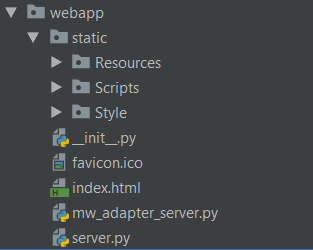
\includegraphics[width=0.33\textwidth]{Dirtree}
  \caption{Directory Tree}
  \label{fig:Dateibaum}
\end{figure}

\paragraph{Sanic}
Sanic ist ein Python 3.6+ Webserver und Webframework, welches den Fokus auf Performanz legt. Durch den Einsatz der im Python 3.5 hinzugefügten 'async/await' Syntax wird der Code nicht-blockierend und schneller.

Das Projekt ist für kleine Projekte ideal, auch ist Python ein grosser Pluspunkt, weshalb wir uns für diese Technologie entschieden haben.

\paragraph{REST API} 
Kommunikation zwischen Client und Server wird mittels einer REST (Representational State Transfer) API (Application-Programming-Interface) gewährleistet. Wir beschränken uns auf die GET und POST Methoden, weil unsere Applikation eine überschaubare Komplexität aufweist.

REST ist eine weit verbreitete API Architektur, welche vor allem im Web Anwendung findet.

\begin{figure}[H] \centering
  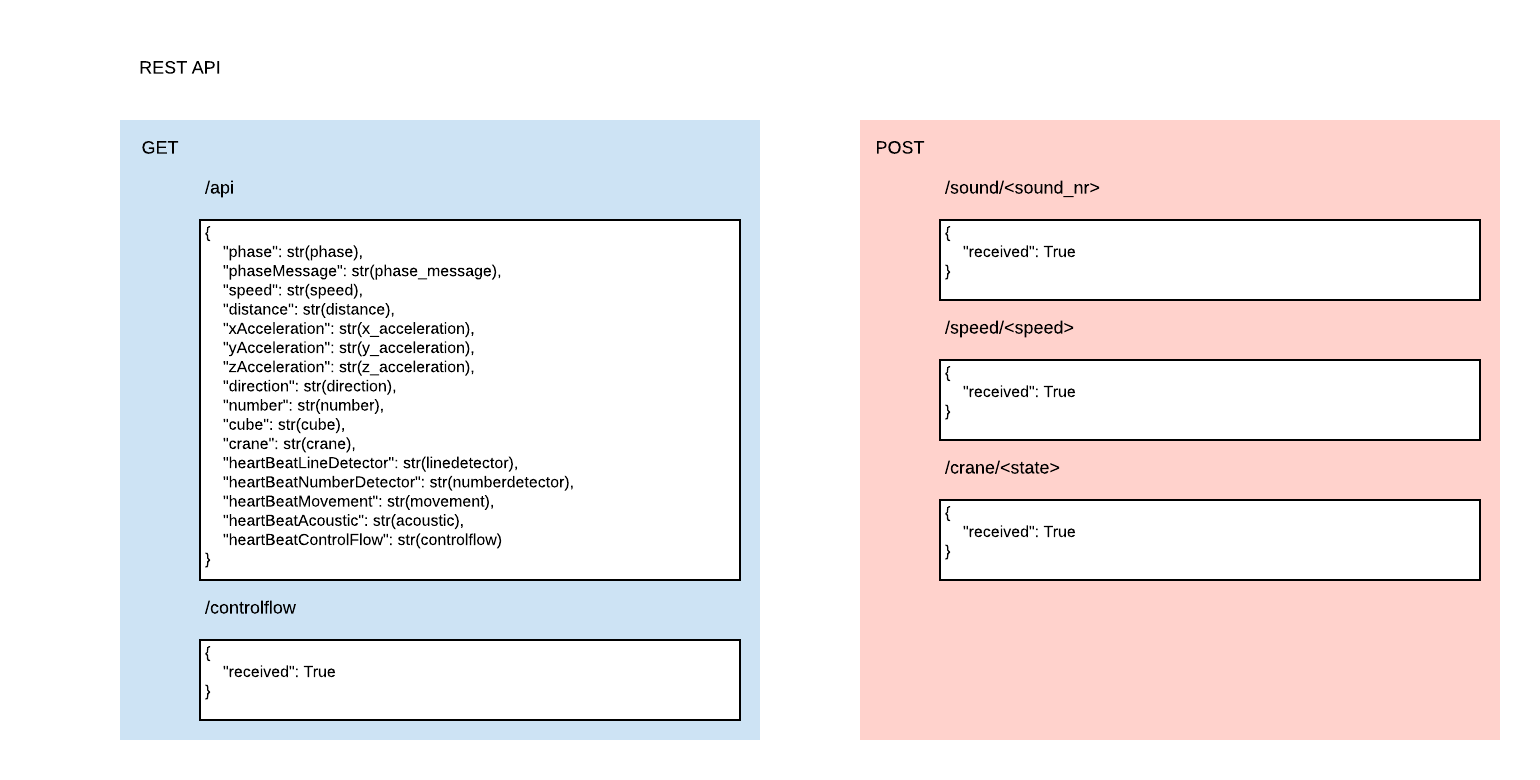
\includegraphics[width=1\textwidth]{RESTAPI}
  \caption{REST API}
  \label{fig:REST API Web}
\end{figure}

\subsubsection{Soll-Ist-Vergleich}
Die WebApp wurde in PREN2 entworfen und entwickelt, somit gibt es keine Erwartungen an diese Komponente. Das Endergebnis entspricht ziemlich genau unseren Vorstellungen.

\subsubsection{Entwicklungsablauf}
Enwurf, sowie erster Prototyp der WebApp wurden von Steve Ineichen anfangs von PREN1 erstellt. Das Hinzufügen immer weiterer Komponenten führte dazu, dass die WebApp im Laufe der Entwicklung kontinuierlich erweitert wurde.

\subsubsection{Testing}
Eine spezifische Testingstrategie für Client oder Server existiert nicht. Die WebApp fungiert als Testingkomponente und ist somit Teststrategie der meisten Komponenten auf dem RasperryPi 3+.
\\
Das Testing erfolgt während des Entwicklungsablaufs automatisch. Wird eine neu eingebundene Komponente auf dem Client simuliert, so wird die Funktionalität der WebApp mitgetestet.

\subsubsection{Reflexion}
Eine Testingkomponente einzuführen war eine tolle Idee und hat sich während der Entwicklung sehr bewährt. Die WebApp liefert eine attraktive Übersicht betreffend den verschiedenen Komponenten.

\end{document}